\documentclass[10pt,a4paper]{article}
%\usepackage{ctex}
\usepackage{CJK}
\usepackage{color}
\usepackage[left=1.2in,right=1.2in,top=1.5in,bottom=1.5in]{geometry} %导入页面边距宏
\usepackage{fancyhdr} %导入页眉页脚宏
\usepackage{lastpage} %引用页数信息
\usepackage{setspace} %行间距
\usepackage{graphicx} %插入图片
\usepackage{amsmath} %数学公式处理 align环境
\usepackage{tikz} %画图
\usepackage{pgfplots} %画图用 axis环境
\usepackage[pdfstartview=FitH,
CJKbookmarks=true,
bookmarksnumbered=true,
bookmarksopen=true,
colorlinks,
pdfborder=001,
linkcolor=blue,
anchorcolor=blue,
citecolor=blue,
]{hyperref} %实现目录和章节的超链接
\hypersetup{hidelinks}

\pagestyle{fancy} %页面样式
\lhead{Chdy} %左页眉
%\chead{\begin{CJK}{UTF8}{gbsn}{\leftmark} \end{CJK}} %中间页眉
\rhead{\begin{CJK}{UTF8}{gbsn}{\leftmark} \end{CJK}} %右页眉
\rfoot{\thepage} 
\cfoot{}

\begin{document}
\begin{CJK}{UTF8}{gbsn}

\author{Dy\footnote{837123564@qq.com}}
\title{Latex}
\date{\today}
\maketitle
\thispagestyle{empty} %去除因maketitle而产生的页码
\newpage
\tableofcontents

\newpage
\section{\color[rgb]{0.2,0.4,0.6} {第一章 Latex的插图与项目符号}}
\subsection{行间距}
\begin{spacing}{2.0} %行间距变为double-space
\paragraph{ \ \ } 在这章介绍如何创建 Qt 的对话框。对话框是程序和用户交互的桥梁,提供了程序和用户之间对话的一种方式。
很多程序都是由一个主窗口,在这个主窗口中包含一个菜单条,多个工具条,和足够多
的对话框。也有些程序本身就是一个对话框,直接相应用户的输入请求。
\par 本章中我们首先会用代码的方式创建我们的第一个对话框,然后用 Qt Designer 工具
创建对话框。Qt Designer 是一个可视化的工具,用它可以更快的创建,修改对话框。
\end{spacing}
\subsection{插图}

	
\begin{figure}[!htb] %图片默认会出现在一页的最顶部,通过参数进行更改,h代表here,放不下就放到top,再放不下就放到bottom
\begin{minipage}[t]{0.48\linewidth} %b表示标题底端对齐,t表示按标题顶端对齐,c表示中间对齐
	\centering %后面的内容全部居中
	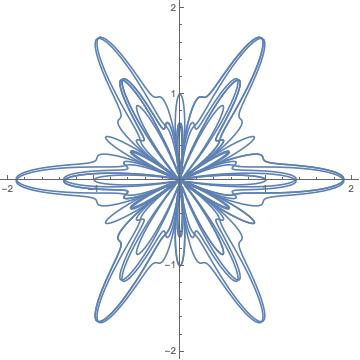
\includegraphics[scale=0.48]{six.jpg} %插入图片并设置缩放,可使用scale=0.x,或者width=0.x乘\textwidth(文字宽度)
	\caption{六角星图}
\end{minipage}
\hfill
\begin{minipage}[t]{0.48\linewidth}
	\centering %后面的内容全部居中
	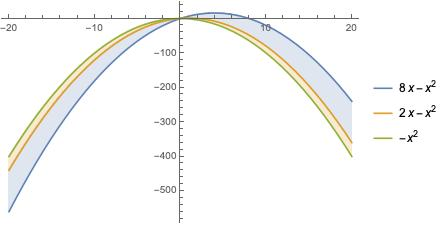
\includegraphics[scale=0.48]{ploy.jpg} %插入图片并设置缩放,可使用scale=0.x,或者width=0.x乘\textwidth(文字宽度)
	\caption{三条线的图}	
\end{minipage}
	
\end{figure}


\subsection{项目符号}
\begin{itemize} %项目符号
	\item yes
\end{itemize}

\begin{enumerate}%项目符号
	\item[一.] A
\end{enumerate}

\subsection{表格}
\begin{table}[!htb] %表格
\centering
	\begin{tabular}{|c|l|r|}
		\hline
		paper & pencil & ruler \\
		\hline
		10\$ & 20\$ & 30\$ \\
		\hline
	\end{tabular}
	\caption{购物表}
\end{table}


\vskip 3 cm %跳过x cm的间距。

\newpage

\section{\color[rgb]{0.2,0.4,0.6} {第二章 数学公式的使用}}

\subsection{行内形式和外部形式}
\paragraph{} 行内形式使用\$x\$符号包围表达式$x$
\paragraph{} 下面是外部形式
$$x^2$$
\[
x^2 + x_2
\]
\subsection{分支形式}
\begin{equation}
	y = \begin{cases}
		1 & x\geq 1\\
		0 & x=0 \\
		-1 & x\leq -1
	\end{cases}
\end{equation}

\subsection{矩阵形式}
\begin{equation}
	y = \left[\begin{array}{ccc}
		1&2&3 \\
		4&5&6 \\
		7&8&9
	\end{array}\right]
\end{equation}

\subsection{方程变换}
\begin{align}
	f &= (x+y)^2 + z^2\nonumber \\
	  &= x^2 + y^2 + 2xy + z^2 \\
	  &= 5\nonumber
\end{align}

\subsection{方程中使用普通文本}
\begin{equation}
	E = \text{ETC} \times 2\sqrt{l_x^2 + l_y^2} \times 0.15
\end{equation}

\subsection{导数}
\begin{equation}
	(\vec{x})'' = -g \hat{z} - \frac{k}{m}|v|^2\hat{v}
\end{equation}

\subsection{求和}
\begin{equation}
	\sum_{i=1}^n f(i)
\end{equation}

\subsection{积分}
\begin{equation}
	\int_0^\infty f(x)\mathrm{d}x
\end{equation}

\subsection{三角函数}
\begin{equation}
	\sin\theta + \cos\theta
\end{equation}

\newpage


\section{\color[rgb]{0.2,0.4,0.6}{画图}}
\subsection{坐标轴}
\begin{figure}[!htb]
\centering
\begin{tikzpicture}
	\begin{axis}[width=270pt,height=200pt,
	xmin=0,xmax=8,ymin=0,ymax=12,
	xlabel={x},ylabel={y}]
		\addplot[color=red,mark=*] table{
		x y
		2 1.2
		3 3.5
		4 2.6
		5 7.8
		6 9.5
		7 2
		};
	\end{axis}
\end{tikzpicture}
\caption{坐标轴}
\end{figure}

\end{CJK}
\end{document}
